\section{Lokation}
Man kan anmode lokation på et væld af måder, f.eks. få fat i den seneste lokation, anmode en enkelt opdatering, anmode flere opdatering. 
Dette afhænger af rettigheder til brug af henholdsvis grov eller fin lokation, og også på andre applikationers anmodninger og forbindelser. Det er muligt at sætte minimum og maksimum tid, men kan ikke garanteres at minimum overholdes. Hyppig opdatering er strømkrævende. 
Data er en lokation (breddegrad, længdegrad, præcision, tidsstempel).

\subsection{Lokation og aktivitet}
Dette kan bruges til at vide hvor brugeren er og hvor meget de bevæger sig (f.eks. til motion).
Derudover kan det også bruges til at vise hvor man opholder sig mest, jævnfør Figur \ref{heatmap}.
\subsection{Nøglelokation}
Man kan finde ud af hvor meget man er ved nogle nøglelokationer, f.eks. hjem eller arbejde og udfra det finde ud af hvor meget man er udenfor hjem. Man kan finde ud af hvor man er oftest (venner, familie, hjem, værtshus).

\begin{figure}[h]
	\centering
	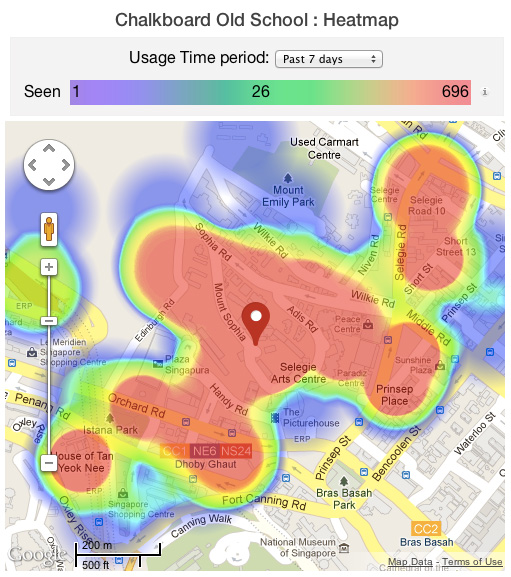
\includegraphics[scale=0.4]{chalkboard-heatmap}
	\caption{Heatmap over lokation.}\label{heatmap}
\end{figure}
